\section{Korma-Curry}
% Linke Seite: Rezept
\textbf{Nur für starke Mägen!}

Zutaten:
\begin{itemize}
    \item 1 Tüte Mandeln (Scheibchen)
    \item 1 rote Zwiebel
    \item 1 Tl Rapsöl
    \item 1/2 Glas Korma-Paste
    \item 200g Schlagsahne
    \item (Beilage) Jasmin-Reis
\end{itemize}

\noindent Zubereitung:

\noindent Mandeln bei mittlerer Hitze in Pfanne anrösten, bis sie gelb-braun
sind. Aus der Pfanne nehmen.

Zwiebel kleinschneiden und in Öl anschwitzen. Korma-Paste dazugeben und kurz
anbraten. Dann mit Wasser ablöschen, Mandeln untermischen, und bei
geschlossenem Deckel ca. 15 Minuten bei geringer Hitze köcheln lassen. Dann
Sahne dazugeben und aufköcheln lassen. Mis Reis servieren.

% Recht Seite: Bild
\newpage
\mbox{}
\vfill
\begin{center}
    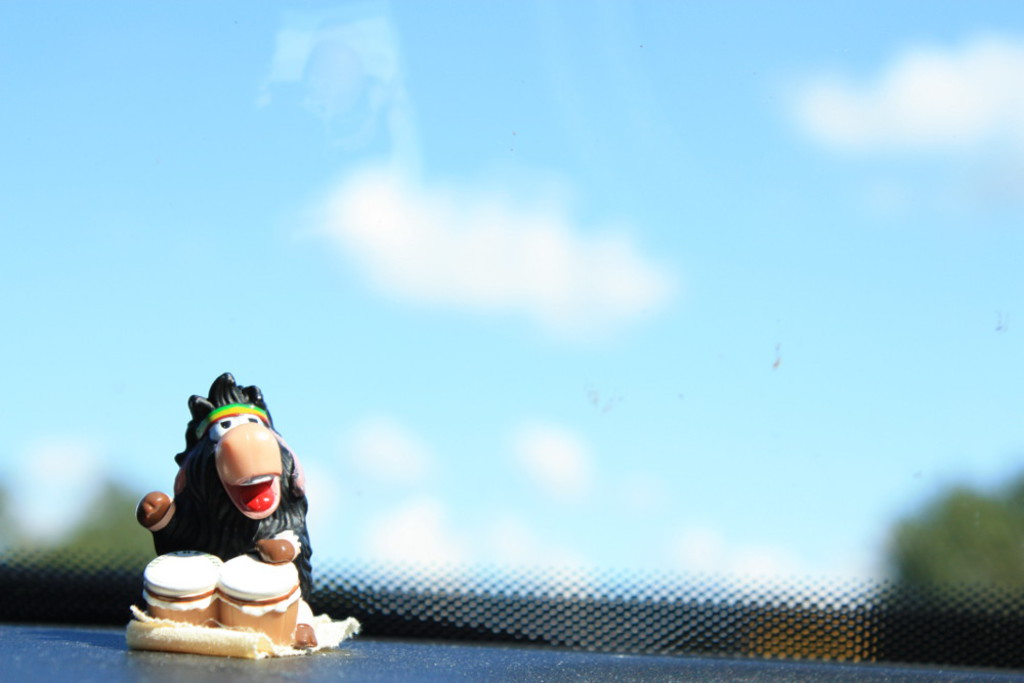
\includegraphics[width=\textwidth]{Korma/IMG_3250._small.jpg}
\end{center}
\vfill
\mbox{ }
\newpage
